\documentclass[a4paper]{article}

\usepackage[linesnumbered, ruled]{algorithm2e}
\usepackage{ tipa }

\usepackage[english]{babel}
\usepackage[utf8]{inputenc}
\usepackage{amsmath}
\usepackage{graphicx}
\usepackage[noend]{algpseudocode}
\usepackage[colorinlistoftodos]{todonotes}
\usepackage{multirow}
\usepackage{parskip}
\usepackage{enumerate}
\usepackage{url}

\setlength{\parindent}{0pt} % no indent in the beginning of a paragraph

% empty set package
\usepackage{amssymb}
\usepackage{tikz}
\usetikzlibrary{automata,positioning}


\title{CSCE 423/823 - Homework 4}
\author{Tian Gao}
\begin{document}
\maketitle

% 1
1.\\
Algorithm:\\
1. Convert G into a network flow graph H, and the capacity of each edge is 1.\\
2. Find the maximum flow f of graph H from u to v.\\
3. If the value of f, $|f|$, is not less than 2, then there are at least two edge-disjoint paths from u to v in G that have no edges in common. 
Otherwise, the statement doesn't hold.\\

Explanation:\\
Since the capacity of each edge in network flow graph H is 1, all the paths in flow f won't share common edges.\\
So the value of f is equal to the number of edge-disjoint paths.\\
So if the value of f is not less than 2, there are at least two edge-disjoint paths from u to v in G that have no edges in common.\\

Time Complexity:\\
step1: $O(V + E)$.\\
step2: $O(VE^2)$.\\
step3: $O(1)$.\\
So in total, the time complexity is $O(VE^2)$.\\

% 2
2.\\
The basic idea of FORD-FULKERSON is to find a augmenting path starting from $s$ in the residual network.\\
Since the paths are always from $s$, the augmenting paths don't include the edges into $s$.\\ 
So augmenting paths don't change even if we delete those edges.\\
Since the augmenting paths don't change, the final maximum flow is the same.\\
So the statement is correct.\\

% 3
3.\\
The flow conservation property is satisfied but the capacity constraint is not satisfied.\\
Since G is a flow network, if $(u,v) \in E, (v, u) \notin E$.\\
We have
\begin{equation}
	(f+f')(u,v)=\left\{
	\begin{array}{lr}
		f(u,v) + f'(u,v) - f'(v,u) = f(u,v) + f'(u,v), & if (u, v) \in E \\
		0.                                             &                 \\
	\end{array}
	\right.
\end{equation}

\begin{align}
	\sum_{v \in V}(f+f')(u,v) & = \sum_{v \in V} f(u,v) + f'(u,v)               \\
	                          & = \sum_{v \in V} f(u,v) + \sum_{v \in V}f'(u,v) \\
	                          & = \sum_{v \in V} f(v,u) + \sum_{v \in V}f'(v,u) \\
	                          & = \sum_{v \in V} f(v,u) + f'(v,u)               \\
	                          & = \sum_{v \in V}(f+f')(v,u)                     
\end{align}
So the flow conservation property is satisfied.\\

Consider the graph G below:\\
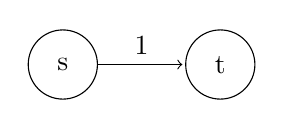
\begin{tikzpicture}[shorten >=1pt,node distance=2cm,on grid,auto] 
	\node[state] (s)   {s}; 
	\node[state] (t) [right=of s] {t}; 
	\path[->] 
	(s) edge  node {1} (t)
	;
\end{tikzpicture}\\
There is only one flow. \\
So $f=f'$ and $f(s, t) = f'(s, t) = 1$, and $c(s,t) = 1$.\\
$(f+f')(s,t) = f(s, t) + f'(s, t) = 2 > 1 = c(s,t)$.\\
So the capacity constraint is not satisfied.\\

% 4
4.\\
\begin{algorithm}[H]
	\caption{isMinCutUniq(G, C, s, t)}
	volC = getVol(C) //get $|C|$, the volume of cut C \;
	\For{each edge e = (u, v) $\in$ G.E}
	{
		G1 = genNewGraph(G, (u, v))\;
		C1 = getMinCut(G1, s, t)\;
		volC1 = getVol(C1)\;
		\If{volC == volC1}
		{
			return false
		}
		return true
	}
\end{algorithm}

\begin{algorithm}[H]
	\caption{genNewGraph(G, e): generate new graph G1 increasing c(u, v) by 1}
	G1 = G\;
	$c_{G1}(u, v) = c_{G1}(u, v) + 1$\;
	return G1\;
\end{algorithm}

Explanation:\\
In the new graph G1 increasing capacity of each edge c(u, v) by 1, we are looking for a min-cut C1 with the same volume as C. \\
If there exist such a C1, C1 is another min-cut in G and C1 $\neq$ C.\\
Then the min-cut is not unique.\\

Time Complexity:\\
In the algorithm, each loop cost polynomial time to generate a new graph, compute a min-cut and get the volume of a min-cut.\\
And there are $|E|$ loops.\\
So the total time complexity is polynomial\;

% 5
5.\\
1). G only has an X-saturating matching. \\
$\Leftrightarrow$
For any $W \subseteq X$, we have $|N_G(W)| \geqslant |W|$ where $|N_G(W)|$ denotes the neighborhood of W in G. \\
Explanation:\\
According to Hall's marriage theorem(ref[1]), $|N_G(W)| \geqslant |W|$ is a a necessary and sufficient condition for the property that G only has an X-saturating matching.\\
\\
2). G only has a Y-saturating matching.\\
$\Leftrightarrow$
For any $W \subseteq Y$, we have $|N_G(W)| \geqslant |W|$ where $|N_G(W)|$ denotes the neighborhood of W in G. \\
Explanation:\\
According to Hall's marriage theorem(ref[1]), $|N_G(W)| \geqslant |W|$ is a a necessary and sufficient condition for the property that G only has a Y-saturating matching.\\
\\
3). G has a perfect matching.\\
$\Leftrightarrow$
For any $W \subseteq S$, we have $|N_G(W)| \geqslant |W|$ where $|N_G(W)|$ denotes the neighborhood of W in G where S is the smaller one of A and B. \\
Explanation:\\
According to Hall's marriage theorem(ref[1]), $|N_G(W)| \geqslant |W|$ is a a necessary and sufficient condition for the existence of a perfect matching in the graph.\\

Reference:\\
1. En.wikipedia.org. (2018). Hall's marriage theorem. [online] Available at: https://en.wikipedia.org/wiki/Hall%27s_marriage_theorem [Accessed 6 Aug. 2018].\\
\\

% 6
6.\\
The network flow formulation can be develop using the following rule:\\
1. Set a source vertex s and n vertices for n men. Set n edges connected the source vertex with each vertex for men. The capacity of each edge is 1.\\
2. Set a sink vertex t and n vertices for n women. Set n edges connected the sink vertex with each vertex for women. The capacity of each edge is 1.\\
3. Set two vertices for each matchmakers. Set an edge between these two vertices with the capacity of $c_i$.
One of the two vertices connects the men vertices that the matchmaker knows, and the other vertex women connects the vertices that the matchmaker knows.\\

After developing the network flow, Ford-Fulkerson algorithm can be used to find the maximum number of marriages.\\
In the maximum flow f, each path from s to t is a marriage. Since the capacity of the edge between vertices $b_i$ is $c_i$, the constraint that $b_i$ can arrange at most $c_i$ marriages is also satisfied.\\
So the value of maximum flow $|f|$ is the maximum number of marriages.\\

\end{document}
